%======================================================================
\subsection{MOD-07 plan: frames, lumber and weld beads on FrameForge (23 Oct 2026, approved 24 Oct)}\label{sec:mod07-plan}
%======================================================================

\eref{MOD-07} gives BruceWorx structural frames: members swept along sketch lines from a profile library, mitres and
trims, a cut list, dimensional lumber with board feet, and weld beads that show as weld symbols on drawings. This plan
compares the open-source frame add-ons, reports a spike in this build, gives the cut-length, board-foot and weld theory,
and proposes adopting FrameForge with a thin BruceWorx layer.

\paragraph{Your answers (23 Oct).}
\begin{center}
\small
\begin{tabularx}{\linewidth}{@{}lX@{}}
\toprule
Question & Answer\\
\midrule
Start from & An existing open-source frame add-on: evaluate FrameForge and other maintained candidates (maintenance,
  licence, FreeCAD~1.1).\\
Metal profiles & 2020/2040 extrusion, square and round tube, angle, flat bar.\\
Lumber & $2\times4$, $2\times6$, \ldots{} at \emph{actual} sizes, cut list in board feet; LumberCAD as a reference.\\
Welds & Weld beads (fillet) between members, with weld symbols on drawings.\\
\bottomrule
\end{tabularx}
\end{center}

%----------------------------------------------------------------------
\subsubsection*{1. The candidates}

Every frame-related add-on in FreeCAD's Addon Manager catalogue was cloned into a scratch folder, plus MetalWB (from its
GitLab mirror), the ancestor of FrameForge. ``12\,mo'' counts commits since 23 Oct 2025.
\begin{center}
\footnotesize
\begin{tabularx}{\linewidth}{@{}>{\raggedright\arraybackslash}p{2.5cm}>{\raggedright\arraybackslash}p{2.9cm}>{\raggedright\arraybackslash}p{1.7cm}cX@{}}
\toprule
Add-on & Licence (file / metadata) & Last commit & 12\,mo & What it is\\
\midrule
\textbf{FrameForge} 0.2.1 & LGPL-3.0 / LGPL-3.0-only$^{a}$ & 14 Apr 2026$^{b}$ & 226 & Members from sketch edges,
  metal, aluminium and wood libraries, trim, end mitre, cut-outs, BOM, cut list with stock nesting, part IDs,
  TechDraw balloons\\
freecad\_frame 0.1.1 & LGPL-2.1-or-later & 1 Aug 2026 & 17 & Beam, mitre, plane and shape cut; profile must be a
  face in the XY plane; no library, no cut list; one author\\
StandardBeams 1.0.0 & LGPL-2.1 code, CC-BY-SA icons & 23 Jan 2026 & 33 & Inserts standard sections (I, H, C, L,
  tubes) with section properties; no frames\\
EasyProfileFrame 0.0.1 & LGPL-3.0-or-later & 11 Apr 2025 & 0 & Profiles on edges; dormant\\
MetalWB 0.0.1 & LGPL-2.1 / ``GPLv2'' & 21 Feb 2023 & 0 & FrameForge's ancestor; dormant, not in the catalogue\\
Woodworking 4.0 & MIT & 6 Oct 2026 & 110 & Furniture panels, joinery, cut list (\emph{getDimensions}); not
  frames, but a reference for wood cut lists\\
Timber & GPL-2 & 11 Jul 2019 & 0 & Timber beams and Eurocode~5 check; dormant\\
\bottomrule
\end{tabularx}\\[2pt]
{\footnotesize $^{a}$ README says ``GPLv3''; two files carry LGPL-2.1-or-later headers (inherited from MetalWB).
$^{b}$ \code{main}; the \code{develop} branch moved last on 16 Jun 2026. 36 open issues and pull requests, the newest
from 8 Oct 2026, unanswered.}
\end{center}
\textbf{FrameForge is the only maintained add-on that does the whole job}: it is the one to adopt. Its weak point is
maintenance: one main author, quieter since April. None of the candidates has weld beads or US lumber.

%----------------------------------------------------------------------
\subsubsection*{2. What was tested (23 Oct)}

FrameForge (commit \code{38511e7}) loaded in this build with \code{-M}; its 12 commands register without leaving Part
Design, like SheetMetal's. The spike drew a $280\times180$ centre-line rectangle, put four $20\times20\times2$ square
tubes (EN~10219, 1.05\,kg/m) on its edges, mitred all four corners with \emph{End Miter}, and ran FrameForge's BOM and
cut list (1\,000\,mm stock, 3\,mm kerf).
\begin{center}
\small
\begin{tabularx}{\linewidth}{@{}Xll@{}}
\toprule
Check & Default (as installed) & \emph{Pre-extend} on\\
\midrule
Member lengths before mitre & 280, 180 & 320, 220\\
Members after mitre: valid, overlap with neighbours & 4 valid, 0\,mm$^3$ & 4 valid, 0\,mm$^3$\\
Cut list length (long point), angles & \textbf{280, 180}; 45/45 & \textbf{300, 200}; 45/45\\
Frame fused: solids, volume & 1 solid, 119\,495.74\,mm$^3$ & 1 solid, 123\,003.18\,mm$^3$\\
Expected volume $A\sum L_c$ ($A=133.699$\,mm$^2$, $\sum L_c = 920$) & \multicolumn{2}{l}{123\,003.1\,mm$^3$}\\
Stock (1\,000\,mm, kerf 3) & 1 stick, 932 used & 2 sticks (1\,012 needed)\\
Profile, mitre, recompute times & \multicolumn{2}{l}{0.04\,s for 4 members, 0.09\,s for 4 mitres}\\
$2\times4$ wood member, 8\,ft (38.1 $\times$ 88.9 $\times$ 2\,438.4) & \multicolumn{2}{l}{valid; 8\,259\,080\,mm$^3$ = 504\,in$^3$ exactly}\\
\bottomrule
\end{tabularx}
\end{center}

\begin{figure}[!htbp]
\centering
\begin{minipage}[b]{0.38\linewidth}\centering
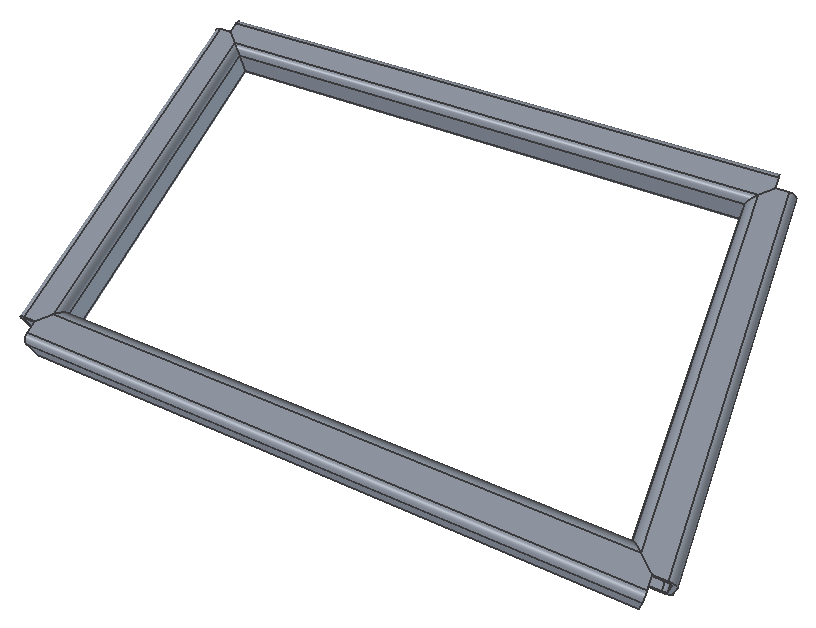
\includegraphics[width=\linewidth]{fig/mod07_frame_default.png}\\{\footnotesize (a) default}
\end{minipage}\hfill
\begin{minipage}[b]{0.5\linewidth}\centering
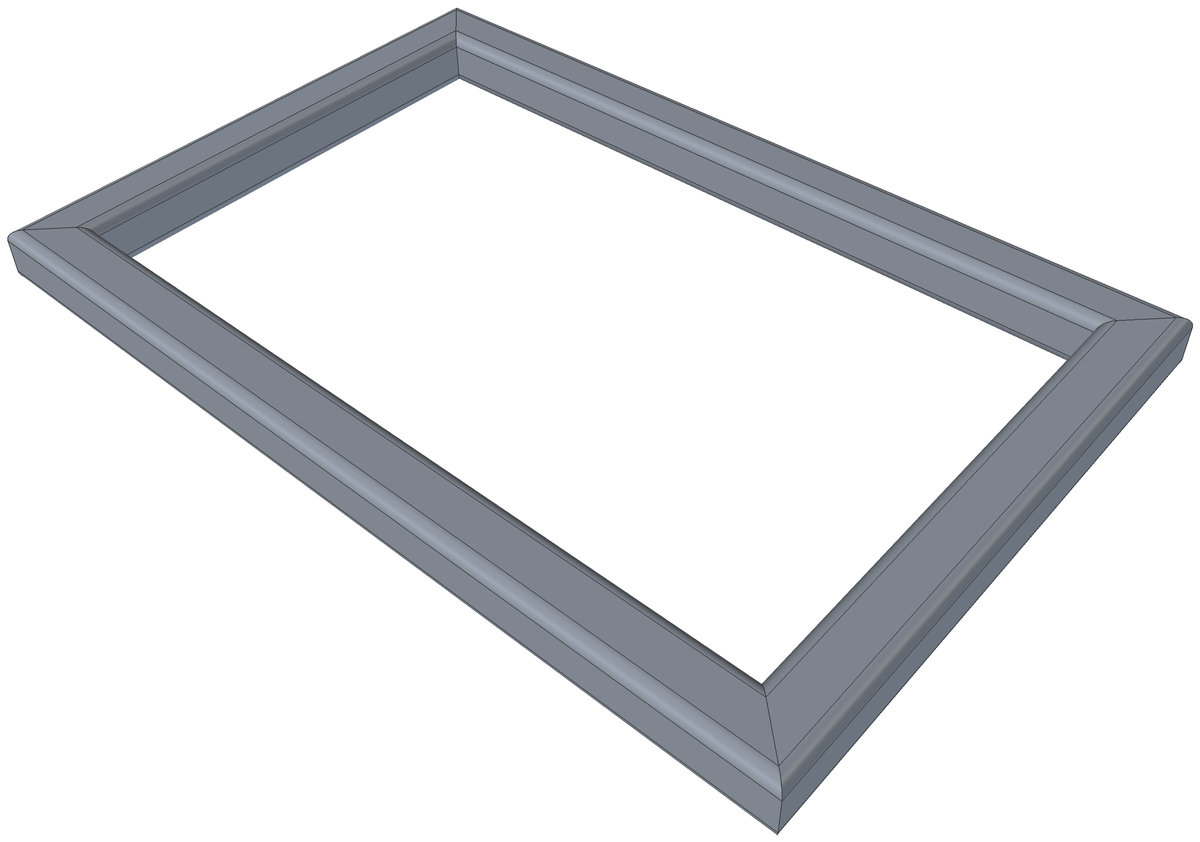
\includegraphics[width=\linewidth]{fig/mod07_frame_mitred.png}\\{\footnotesize (b) pre-extend}
\end{minipage}\\[6pt]
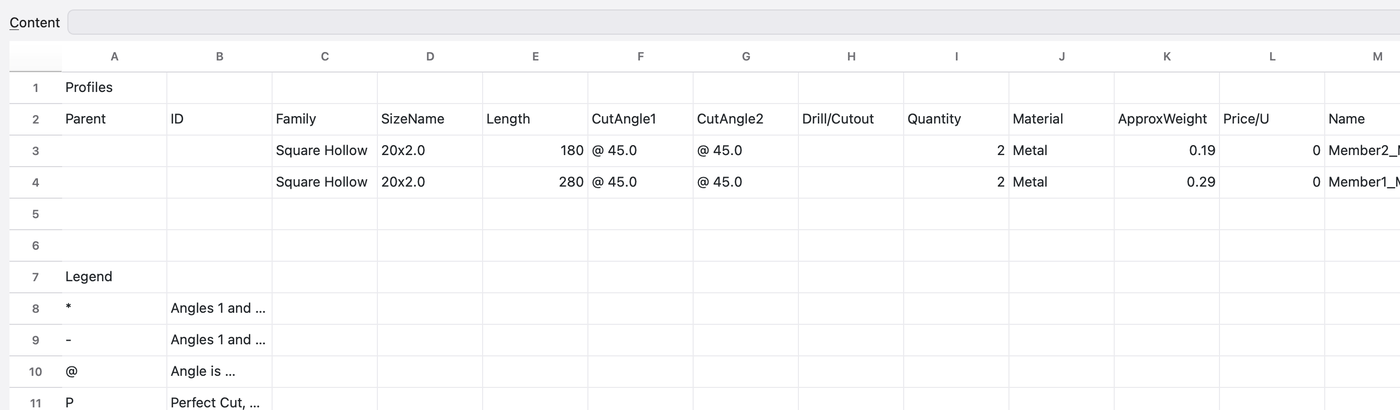
\includegraphics[width=\linewidth]{fig/mod07_bom_sheet.png}\\{\footnotesize (c) FrameForge's BOM for (a)}\\[4pt]
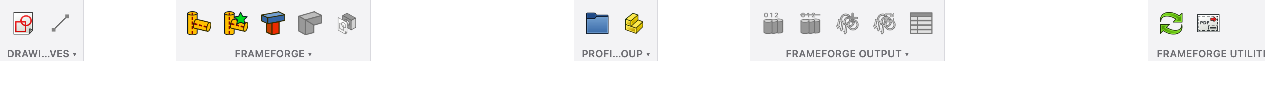
\includegraphics[width=0.85\linewidth]{fig/mod07_toolbar.png}\\{\footnotesize (d) FrameForge's toolbars}
\caption{The FrameForge spike in this build, light theme. (a)~With the default settings each tube stops at the
corner point, so the mitre leaves the outer corners open. (b)~With \emph{Pre-extend} the corners close and the frame is
one solid of exactly $A\sum L_c$. (c)~The BOM of (a) lists the centre-line lengths 280/180, so stock would be short
by 20\,mm per member. (d)~Its 16 toolbar buttons (12 commands of its own).}
\label{fig:mod07-spike}
\end{figure}

\paragraph{Findings.}
\begin{enumerate}[nosep]
  \item \textbf{The default cuts the wrong lengths.} Without \emph{Pre-extend} (off by default) a member ends at the
        corner point and the mitre removes the half-wedge on its inner side; the four corners miss
        $4\times877 = 3\,507$\,mm$^3$ and the cut list says 280 where the saw must cut 300. Our layer turns
        \emph{Pre-extend} on, and our cut list checks lengths against the theory below.
  \item \textbf{The rest is sound}: mitres are exact (no overlap, one valid solid, volume to 0.1\,mm$^3$), cut angles
        are reported per end, and identical members are grouped with quantities.
  \item \textbf{No inch sizes and no US lumber.} The libraries are EN metal profiles, 20-series V-slot and T-slot
        (20$\times$20 to 20$\times$80), and French metric wood sections. Round tube exists only as DN pipe.
  \item \textbf{The BOM is a spreadsheet in the document}, keyed by labels. It is not the assembly BOM
        (\eref{ASM-04}) and knows nothing about board feet or welds.
\end{enumerate}

%----------------------------------------------------------------------
\subsubsection*{3. Theory}

\paragraph{Cut length at a mitre.}
\begin{figure}[!htbp]
\centering
\begin{tikzpicture}[scale=1.0,>=Stealth]
  \def\h{0.6}
  \fill[black!8] (-\h,-\h) -- (8,-\h) -- (8,\h) -- (\h,\h) -- cycle;
  \fill[black!14] (-\h,-\h) -- (\h,\h) -- (\h,3) -- (-\h,3) -- cycle;
  \draw[thick] (-\h,-\h) -- (8,-\h) (\h,\h) -- (8,\h) (-\h,-\h) -- (-\h,3) (\h,\h) -- (\h,3);
  \draw[thick,bwred] (-\h,-\h) -- (\h,\h);
  \draw[bworange,dash dot] (0,0) -- (8.3,0) (0,0) -- (0,3.2);
  \fill (0,0) circle (1.5pt) node[left=2pt,font=\scriptsize] {$\mathbf c$};
  \draw[<->] (\h,1.2) -- (8,1.2) node[midway,above,font=\scriptsize] {short point: $L_c - \tfrac{w}{2}\tan\tfrac{\alpha}{2}$ at this end};
  \draw[<->] (0,-1.2) -- (8,-1.2) node[midway,below,font=\scriptsize] {$L_c$: centre line};
  \draw[<->] (-\h,-2.1) -- (8,-2.1) node[midway,below,font=\scriptsize] {long point: $L_c + \tfrac{w}{2}\tan\tfrac{\alpha}{2}$ at this end};
  \draw[densely dotted] (0,-0.1) -- (0,-1.3) (-\h,-\h) -- (-\h,-2.2);
  \draw[<->] (8.5,-\h) -- (8.5,\h) node[midway,right,font=\scriptsize] {$w$};
  \draw[bwred,<-] (0.15,0.15) -- (1.6,-0.3) node[right,font=\scriptsize] {mitre plane, normal $\hat{\mathbf d}_1+\hat{\mathbf d}_2$};
\end{tikzpicture}
\caption{One mitred corner (plan view): $\alpha$ is the turn between members, $90^\circ$ here; the cut is $\alpha/2$ from
square.}
\label{fig:mod07-mitre}
\end{figure}
With the skeleton on the centre lines, a member between two mitred corners of turn $\alpha$ has
\[
  L_{\text{long}} = L_c + 2\cdot\tfrac{w}{2}\tan\tfrac{\alpha}{2},\qquad
  L_{\text{short}} = L_c - 2\cdot\tfrac{w}{2}\tan\tfrac{\alpha}{2},
\]
where $w$ is the profile's width in the plane of the turn. A saw is set from the long point, so the cut list gives
$L_{\text{long}}$ (and the short point as a check). For the spike, $w=20$, $\alpha=90^\circ$: $280 \rightarrow 300/260$
and $180 \rightarrow 200/160$, the numbers of Figure~\ref{fig:frame}. A \emph{butt} end against a member of width
$w'$ gives $L = L_c - \tfrac{w'}{2}$ at that end (the other member runs through), and a \emph{cope} keeps $L_c$ but
removes the other member's section. A mitred frame conserves material at the centre line: its volume is
$A\sum L_c$, which is why the pre-extended spike matched to 0.1\,mm$^3$ and the default did not. The stock needed is a
bin-packing problem: parts of length $L_i + \kappa$ (kerf $\kappa$) into sticks of length $S$; FrameForge uses
best-fit decreasing, within $\tfrac{11}{9}\mathrm{OPT}+\tfrac{6}{9}$ sticks, more than enough for a shop cut list.

\paragraph{Board feet, nominal and actual.} A board foot is $12\times12\times1$\,in, so
\[
  \mathit{BF} = \frac{t_{\text{in}} \times w_{\text{in}} \times L_{\text{ft}}}{12}.
\]
US softwood lumber is sold and priced by its \emph{nominal} size, while the dressed (dry, surfaced four sides) piece is
smaller (American Softwood Lumber Standard, PS~20): $\tfrac12$\,in less for nominal sizes up to 6\,in, $\tfrac34$\,in
less from 8\,in, and 1-by boards are $\tfrac34$\,in thick.
\begin{center}
\footnotesize\setlength{\tabcolsep}{4pt}
\begin{tabular}{@{}lcccccccc@{}}
\toprule
Nominal & $1\times4$ & $2\times2$ & $2\times4$ & $2\times6$ & $2\times8$ & $2\times10$ & $2\times12$ & $4\times4$\\
Actual, in & $\tfrac34\times3\tfrac12$ & $1\tfrac12\times1\tfrac12$ & $1\tfrac12\times3\tfrac12$ & $1\tfrac12\times5\tfrac12$ & $1\tfrac12\times7\tfrac14$ & $1\tfrac12\times9\tfrac14$ & $1\tfrac12\times11\tfrac14$ & $3\tfrac12\times3\tfrac12$\\
Actual, mm & $19\times89$ & $38\times38$ & $38\times89$ & $38\times140$ & $38\times184$ & $38\times235$ & $38\times286$ & $89\times89$\\
\bottomrule
\end{tabular}
\end{center}
A $2\times4\times8$\,ft is $2\cdot4\cdot8/12 = 5.33$ board feet at nominal size, while its wood is
$1.5\cdot3.5\cdot8/12 = 3.50$\,BF (504\,in$^3$, what the spike measured); 66\,\%. The model is drawn at actual size;
the cut list prices in nominal board feet and reports actual volume for mass. Stock comes in even lengths (8 to 16\,ft,
plus $92\tfrac58$\,in precut studs), and a $\tfrac18$\,in kerf is typical for a circular saw.

\paragraph{Fillet welds and the AWS A2.4 symbol.}
\begin{figure}[!htbp]
\centering
\begin{tikzpicture}[scale=0.9,>=Stealth]
  % joint section: plate and upright with fillet
  \begin{scope}[shift={(0,0)}]
    \fill[black!10] (0,0) rectangle (3.2,0.5);
    \fill[black!18] (1.4,0.5) rectangle (1.8,2.6);
    \draw (0,0) rectangle (3.2,0.5) (1.4,0.5) rectangle (1.8,2.6);
    \fill[bworange!70] (1.8,0.5) -- (2.4,0.5) -- (1.8,1.1) -- cycle;
    \draw[<->] (1.8,0.32) -- (2.4,0.32) node[midway,below,font=\scriptsize] {$z$};
    \draw[<->,bwred] (1.8,0.5) -- (2.1,0.8);
    \node[bwred,font=\scriptsize,anchor=north west] at (2.2,-0.05) {throat $a=z/\sqrt2$};
    \node[font=\scriptsize] at (0.7,-0.3) {section};
  \end{scope}
  % symbol
  \begin{scope}[shift={(4.6,1.6)}]
    \draw[thick] (0,0) -- (4.2,0);
    \draw[thick,->] (0,0) -- (-2.3,-0.75);
    \draw (0,0) circle (0.14);
    \draw[thick] (1.5,0) -- (1.5,-0.55) -- (2.05,0) ;
    \node[font=\scriptsize,anchor=east] at (1.45,-0.3) {3};
    \node[font=\scriptsize,anchor=west] at (2.1,-0.3) {80};
    \draw[thick] (4.2,0) -- (4.6,0.35) (4.2,0) -- (4.6,-0.35);
    \node[font=\scriptsize,anchor=west] at (4.65,0) {GMAW};
    \node[font=\scriptsize,anchor=south] at (2,0.1) {(other side: above the line)};
    \node[font=\scriptsize,anchor=north] at (2.3,-0.75) {arrow side: below the line};
  \end{scope}
\end{tikzpicture}
\caption{A 3\,mm fillet weld, 80\,mm long, all around, on the arrow side, made by GMAW (AWS~A2.4). Leg $z$ to the left
of the triangle, length (and pitch) to the right; the circle at the bend of the leader means \emph{all around}; the
tail carries the process or specification.}
\label{fig:mod07-weld}
\end{figure}
A fillet weld of leg $z$ has a triangular section of area $z^2/2$ and throat $a = z\cos45^\circ \approx 0.707\,z$, the
plane on which it fails. In AWS~A2.4 the triangle sits below the reference line for the \emph{arrow side} and above it
for the \emph{other side}, always with its vertical leg on the left; size goes left, length and pitch right
(\code{3 80-150} for an intermittent weld). ISO~2553 uses a solid and a dashed reference line and prefixes the size with
$a$ (throat) or $z$ (leg). Two numbers follow from the bead, and the bead feature reports both: the weld metal
$m = \rho\,\tfrac{z^2}{2}\,L$ (3\,mm all around a $20\times20$ tube, $L\approx73$\,mm with its corner radii:
2.6\,g of steel) and a quick capacity $F = a\,L\,\tau_{\text{allow}}$ (with $0.30\times$ E70 tensile $= 145$\,MPa:
$2.12\times73\times145 = 22$\,kN).

%----------------------------------------------------------------------
\subsubsection*{4. Integration: FrameForge plus a BruceWorx frame layer}

\begin{itemize}[nosep]
  \item \textbf{Bundled like SheetMetal} (\S\ref{sec:mod06-plan}): vendored in \file{package/bruceworx/vendor/FrameForge/},
        pinned, \code{BUILD\_BW\_FRAMEFORGE} option, installed as \file{Mod/FrameForge} with its \file{package.xml}
        (its workbench lives in \file{freecad/frameforge}, a namespace package; loading it this way was tested). No new
        Python packages. Off switch through \code{DisabledAddons}. Licence: LGPL-3.0-only, which FreeCAD's
        ``2.1 or later'' accepts; \file{NOTICE} lists it with the README's ``GPLv3'' discrepancy noted, and the licence
        file is installed under \file{share/doc/BruceWorx/third-party/}.
  \item \textbf{Our layer} (\file{src/Mod/BruceWorx/bruceworx\_frame*.py}), on top of FrameForge's objects, not a fork:
        \begin{itemize}[nosep]
          \item \emph{Structural Member} opens FrameForge's profile panel (figure~\ref{fig:mod07-panel}) with our
                defaults: \emph{Pre-extend} on, members grouped in the frame's part, the BruceWorx profile library.
          \item \emph{Profile library} as JSON files in FrameForge's own format, added to its lists: inch square and
                rectangular tube, \textbf{round tube} (metric and inch), inch angle and flat bar, 20-series T-slot
                $20\times40$, 80/20 1010/1020, and a \textbf{Lumber} material with $1\times$, $2\times$ and $4\times$
                nominal sizes at actual dimensions. Each size carries a nominal name, mass per metre and, for lumber,
                the board-foot factor.
          \item \emph{Cut list}: reads each member's length, end angles, profile and material; checks the long-point
                length against the theory (warning when a member was not pre-extended); groups identical members; packs
                stock with kerf; adds board feet for lumber. It feeds the assembly BOM (\eref{ASM-04}) as one line per
                group with a \code{CutList} sub-table, and a TechDraw table for \eref{DRW-07}. FrameForge's own
                spreadsheet BOM stays available under \emph{more}.
          \item \emph{Fillet Bead}: pick two members (or two faces); the bead is a \code{Part::FeaturePython} that finds
                their intersection edges, sweeps a right triangle of leg $z$ along them (all around or a length, one or
                both sides) and stores size, side, length, pitch, process and all-around. Beads live in a \code{Welds}
                group, count in mass, and are excluded from STEP export and interference checks by default.
          \item \emph{Weld symbols}: on a drawing, \emph{Annotate welds} places a TechDraw leader on each visible bead
                and a \code{TechDraw::DrawWeldSymbol} filled from the bead: TechDraw already ships the AWS fillet tiles
                (\file{Symbols/Welding/AWS/filletUp.svg}, \file{filletDown.svg}), size and length texts, all-around,
                field weld and tail. The symbol follows the vault's drawing standard (ASME $\rightarrow$ AWS~A2.4).
        \end{itemize}
  \item \textbf{One file, many bodies.} Members are bodies in the frame's part with cut-list items, as \eref{MOD-07}
        says, not separate part files.
\end{itemize}

\begin{figure}[!htbp]
\centering
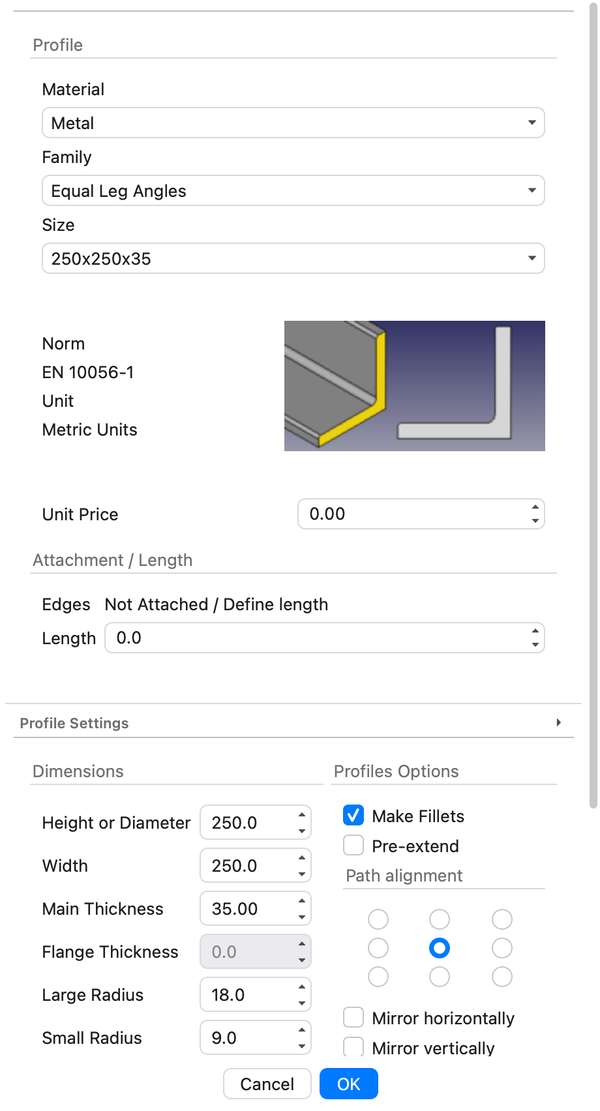
\includegraphics[width=0.3\linewidth]{fig/mod07_profile_panel.png}\hspace{1.5em}
\begin{minipage}[b]{0.55\linewidth}
\caption{FrameForge's \emph{Create Profile} panel in this build: material, family and size lists with a picture, the
dimensions, \emph{Pre-extend}, path alignment (a $3\times3$ anchor grid) and mirroring. Our \emph{Structural Member}
opens it with \emph{Pre-extend} ticked and the BruceWorx library loaded.}
\label{fig:mod07-panel}
\end{minipage}
\end{figure}

\paragraph{The Frame tab.} A new tab in the Design workspace after \emph{Sheet Metal}, with \code{"requires": "FrameForge"}
(SolidWorks calls the same tab \emph{Weldments}; ``Frame'' covers lumber too):
\begin{lstlisting}[language={}]
{ "name": "Frame", "requires": "FrameForge", "groups": [
  { "caption": "Members",
    "commands": ["BruceWorx_StructuralMember", "FrameForge_CreateCustomProfiles",
                 "FrameForge_ParametricLine"],
    "more": ["FrameForge_Link"] },
  { "caption": "Joints",
    "commands": ["FrameForge_EndMiter", "FrameForge_TrimProfiles",
                 "FrameForge_AddExtrudeCutout"] },
  { "caption": "Weld",
    "commands": ["BruceWorx_FilletBead"], "more": ["BruceWorx_WeldList"] },
  { "caption": "Output",
    "commands": ["BruceWorx_CutList"],
    "more": ["FrameForge_CreateBOM", "FrameForge_PopulateIDs",
             "FrameForge_CreateBalloons"] } ] }
\end{lstlisting}

%----------------------------------------------------------------------
\subsubsection*{5. Build order and effort}

\begin{center}
\small
\begin{tabularx}{\linewidth}{@{}lXl@{}}
\toprule
\# & Step & Effort\\
\midrule
1 & Vendor FrameForge (pinned), CMake copy and install, off switch, NOTICE and licence file & 0.5\,d\\
2 & Frame tab and load entries; \emph{Structural Member} with our defaults (pre-extend, grouping) & 0.5\,d\\
3 & Profile library: round tube, inch tube, angle and flat bar, T-slot 2040, 80/20 inch; Lumber at actual size with
  nominal names; tests that every size builds a valid solid & 1.5\,d\\
4 & Cut list: long-point check, grouping, stock packing with kerf, board feet; BOM lines (ASM-04) and a TechDraw
  table (DRW-07); pure logic with tests & 2\,d\\
5 & \emph{Fillet Bead}: intersection edges, triangular sweep, sides, all-around, intermittent; mass and weld list & 2.5\,d\\
6 & \emph{Annotate welds}: leaders and AWS fillet symbols from beads on a drawing & 1.5\,d\\
7 & Acceptance: the frame of Figure~\ref{fig:frame} (cut list 300/200 and legs), a $2\times4$ bench in board feet,
  a drawing with weld symbols; upstream issue and patch for the pre-extend default & 0.5\,d\\
\midrule
 & Total & 9\,d\\
\bottomrule
\end{tabularx}
\end{center}
Steps 1--3 give working frames with correct lengths in two to three days. Step~4 needs the BOM of \eref{ASM-04} for its
BOM lines (the TechDraw table does not). Steps 5--6 are new code with no upstream to lean on.

\paragraph{Risks.} \emph{Maintenance}: FrameForge has one main author and unanswered pull requests since spring; our
layer keeps its own logic (cut list, beads, library) outside FrameForge so a fork, if ever needed, stays small.
\emph{Data migrations}: FrameForge 0.1 $\rightarrow$ 0.2 changed its stored data (its README warns to back up), so each
update is tested on saved frames before it ships. \emph{Bead robustness}: sweeping along intersection edges of filleted
tubes gives short B-spline edges; the bead falls back to a straight sweep on the member's outer edge. \emph{Scale}: a
Python feature per member is fine for tens of members; a 200-member truss needs a timing check (0.01\,s per member
today). \emph{Toponaming}: members attach to sketch edges by name, so editing the skeleton can renumber them, as with
any FreeCAD feature.

%----------------------------------------------------------------------
\paragraph{Your answers to the questions below (24 Oct).} All eight as recommended. 1: \textbf{adopt FrameForge and
layer} our work on it; the pre-extend fix and the inch libraries go upstream; a fork only if upstream stays silent and
its objects must change. 2: frames on member \textbf{centre lines}, pre-extend on. 3: \textbf{nominal} board feet for
the board-foot column and cost, \textbf{actual} volume for mass, both shown. 4: stock lengths 8, 10, 12, 14, 16\,ft
plus $92\tfrac58$\,in studs, kerf $\tfrac18$\,in, as per-vault settings next to the sheet-metal rules. 5: weld beads
as \textbf{solids} in a \code{Welds} group, counted in mass, left out of STEP export and interference checks unless
switched on. 6: weld symbols follow \textbf{the vault's drawing standard}, AWS built first. 7: 20-series metric plus
80/20 1010 and 1020. 8: the tab is called \emph{Frame}. Building started 24 Oct.

\subsubsection*{Questions before MOD-07 starts}

\begin{enumerate}
  \item \textbf{Adopt or fork.} Bundle FrameForge as is and put our work in a separate BruceWorx layer, or fork it now?\\
        \emph{Recommendation:} adopt and layer; send the pre-extend fix and the inch libraries upstream; fork only if
        upstream stays silent and we need to change its objects.
  \item \textbf{Skeleton lines.} Draw frames on member centre lines (with pre-extend on), or on outer edges?\\
        \emph{Recommendation:} centre lines; the cut list then follows the formulas above and matches
        Figure~\ref{fig:frame}.
  \item \textbf{Board feet.} Price lumber by nominal board feet (the trade convention) and give actual volume for mass,
        or use actual volume for both?\\
        \emph{Recommendation:} nominal for the board-foot column and cost, actual for mass, both shown.
  \item \textbf{Lumber stock and kerf.} Default stock lengths 8, 10, 12, 14, 16\,ft plus $92\tfrac58$\,in studs, kerf
        $\tfrac18$\,in?\\
        \emph{Recommendation:} yes, as per-vault settings next to the sheet-metal rules.
  \item \textbf{Weld beads as solids.} Model beads as solids (mass, pictures) or keep welds as symbols only?\\
        \emph{Recommendation:} solids in a \code{Welds} group, counted in mass, left out of STEP export and
        interference checks unless switched on.
  \item \textbf{Symbol standard.} AWS~A2.4 only, or follow the vault's drawing standard (AWS for ASME vaults, ISO~2553
        for ISO vaults)?\\
        \emph{Recommendation:} follow the vault's standard; build AWS first.
  \item \textbf{Extrusion families.} Which aluminium systems do you use: 20-series V-slot/T-slot (metric), 80/20 inch
        (1010/1020), or others (Misumi, Item)?\\
        \emph{Recommendation:} 20-series metric (in FrameForge already) plus 80/20 1010 and 1020.
  \item \textbf{The tab's name.} \emph{Frame} (covers lumber) or \emph{Weldments} (SolidWorks)?\\
        \emph{Recommendation:} \emph{Frame}.
\end{enumerate}
